\exercise

Let us given the symbols and their probabilities: $p_a = p_b = 0.1$, $p_c =
0.2$, $p_d = p_e = 0.11$, $p_f = 0.38$.
%
\begin{enumerate}

  \item Compute the Huffman code for this distribution.

  \item Compute the Canonical variant of the Huffman code, indicating how do you
  compute the canonical codewords.

  \item Decode the first 3 symbols of the coded sequence $10001011011100\dots$

\end{enumerate}

\solution

\begin{enumerate}
  \item \autoref{fig:huffman-tree} shows the Huffman tree of the given distribution. The resulting codewords are
  %
  \begin{center}
    \begin{tabular}{c||c|c|c|c|c|c}
    $\sigma$ &  $a$ & $b$ & $c$ & $d$ & $e$ & $f$ \\\hline
    $C_\sigma$ &  000 & 001 & 01 & 100 & 101 & 11 \\
    \end{tabular}
  \end{center}
  %
  \begin{figure}[t]
    \centering
    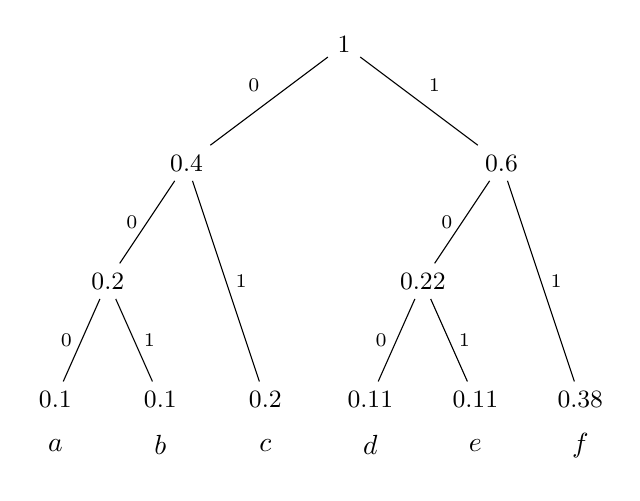
\begin{tikzpicture}[
      grow=down,
      every node/.style={},
      level/.style={sibling distance = 4cm/#1, level distance = 1.5cm}
    ]
    \node {\small 1}
    child {
      node (L) {\small 0.4}
      child {
        node {\small 0.2}
        child {
          node[label={[minimum size = 2em, inner sep=0, text centered]below:{$a$}}] {\small 0.1}
          edge from parent[-] node[left] {\scriptsize 0}
        }
        child {
          node[label={[minimum size = 2em, inner sep=0, text centered]below:{$b$}}] {\small 0.1}
          edge from parent[-] node[right] {\scriptsize 1}
        }
        edge from parent[-] node[left] {\scriptsize 0}
      }
      child {
        node[draw=none] {}
        child {
          node[label={[minimum size = 2em, inner sep=0, text centered]below:{$c$}}] {\small 0.2}
          edge from parent[draw=none]
          edge[-] node[right] {\scriptsize 1} (L)
        }
        edge from parent[draw=none]
      }
      edge from parent[-] node[above left] {\scriptsize 0}
    }
    child {
      node (R) {\small 0.6}
      child {
        node {\small 0.22}
        child {
          node[label={[minimum size = 2em, inner sep=0, text centered]below:{$d$}}] {\small 0.11}
          edge from parent[-] node[left] {\scriptsize 0}
        }
        child {
          node[label={[minimum size = 2em, inner sep=0, text centered]below:{$e$}}] {\small 0.11}
          edge from parent[-] node[right] {\scriptsize 1}
        }
        edge from parent[-] node[left] {\scriptsize 0}
      }
      child {
        node[draw=none] {}
        child {
          node[label={[minimum size = 2em, inner sep=0, text centered]below:{$f$}}] {\small 0.38}
          edge from parent[draw=none]
          edge[-] node[right] {\scriptsize 1} (R)
        }
        edge from parent[draw=none]
      }
      edge from parent[-] node[above right] {\scriptsize 1}
    };
    \end{tikzpicture}

    \caption{Huffman tree for $\Sigma = \{ a, b, c, d, e, f \}$.}

    \label{fig:huffman-tree}
  \end{figure}

  \item We first create Canonical Huffman data structures, which are the
  following
  %
  \begin{center}
    \begin{tabular}{|r||c|c|c|}
      \multicolumn{1}{r}{} & \multicolumn{1}{c}{\tiny 1} & \multicolumn{1}{c}{\tiny 2} & \multicolumn{1}{c}{\tiny 3} \\ \hline
      \tt num & 0 & 2 & 4 \\ \hline
      \tt sym &   & $c$ & $a$ \\
              & & $f$ & $b$ \\
              & & & $d$ \\
              & & & $e$ \\ \hline
      \tt fc  & 2 & 2 & 0 \\ \hline
    \end{tabular}
  \end{center}
  %
  where, for each $\ell$, $\text{\tt num}[\ell]$ represents the number of
  codewords of size $\ell$ in the classical Huffman coding (i.e., the one in the
  previous point), $\text{\tt sym}[\ell]$ represents the ordered list of symbols
  of size $\ell$, and $\text{\tt fc}[\ell]$ the first codeword (in decimal
  representation) between the ones having size $\ell$. To compute this last
  array, we use the recursive formula $$\text{\tt fc}[\ell] =
  \frac{1}{2}(\text{\tt fc}[\ell + 1] + \text{\tt num}[\ell + 1])$$ having as
  base case $\text{\tt fc}[\ell_\text{max} = 3] = 0$. The Canonical Huffman
  codewords will be assigned incrementally to each symbol in $\text{\tt
  sym}[\ell]$ starting from $\text{\tt fc}[\ell]$. The resulting codewords are
  %
  \begin{center}
    \begin{tabular}{c||c|c|c|c|c|c}
    $\sigma$ &  $a$ & $b$ & $c$ & $d$ & $e$ & $f$ \\\hline
    $C_\sigma$ &  000 & 001 & 10 & 010 & 011 & 11 \\
    \end{tabular}
  \end{center}

  \item The first three codewords are $c$, $b$, $e$:
  $$\underbracket{10}_c\underbracket{001}_b\underbracket{011}_e011100\dots$$
  %
  \begin{enumerate}
    \item $l \gets 1$, $v \gets 1$
    %
    \begin{itemize}
      \item $v < \text{\tt fc}[l] \implies v \gets 2 \times v + 0 = 2,\ l \gets l + 1 = 2$
      \item $v \ge \text{\tt fc}[l] \implies \text{\bf output \tt sym}[l, v - \text{\tt fc}[l]] = c$
    \end{itemize}

    \item $l \gets 1$, $v \gets 0$
    %
    \begin{itemize}
      \item $v < \text{\tt fc}[l] \implies v \gets 2 \times v + 0 = 0,\ l \gets l + 1 = 2$
      \item $v < \text{\tt fc}[l] \implies v \gets 2 \times v + 1 = 1,\ l \gets l + 1 = 3$
      \item $v \ge \text{\tt fc}[l] \implies \text{\bf output \tt sym}[l, v - \text{\tt fc}[l]] = b$
    \end{itemize}

    \item $l \gets 1$, $v \gets 0$
    %
    \begin{itemize}
      \item $v < \text{\tt fc}[l] \implies v \gets 2 \times v + 1 = 1,\ l \gets l + 1 = 2$
      \item $v < \text{\tt fc}[l] \implies v \gets 2 \times v + 1 = 3,\ l \gets l + 1 = 3$
      \item $v \ge \text{\tt fc}[l] \implies \text{\bf output \tt sym}[l, v - \text{\tt fc}[l]] = e$
    \end{itemize}
  \end{enumerate}

\end{enumerate}
